\documentclass[utf8]{FrontiersinHarvard} % for articles in journals using the Harvard Referencing Style (Author-Date), for Frontiers Reference Styles by Journal: https://zendesk.frontiersin.org/hc/en-us/articles/360017860337-Frontiers-Reference-Styles-by-Journal
%\documentclass[utf8]{FrontiersinVancouver} % for articles in journals using the Vancouver Reference Style (Numbered), for Frontiers Reference Styles by Journal: https://zendesk.frontiersin.org/hc/en-us/articles/360017860337-Frontiers-Reference-Styles-by-Journal
%\documentclass[utf8]{frontiersinFPHY_FAMS} % Vancouver Reference Style (Numbered) for articles in the journals "Frontiers in Physics" and "Frontiers in Applied Mathematics and Statistics" 

%\setcitestyle{square} % for articles in the journals "Frontiers in Physics" and "Frontiers in Applied Mathematics and Statistics" 
\usepackage{url,hyperref,lineno,microtype,subcaption}
\usepackage[onehalfspacing]{setspace}

\linenumbers
% \documentclass[draft]{agujournal2019}
% \usepackage{url}
% \usepackage{lineno}
% \usepackage{soul}
\usepackage{minted}

\def\keyFont{\fontsize{8}{11}\helveticabold }
\def\firstAuthorLast{Shumko {et~al.}}
\def\Authors{M. Shumko\,$^{1,2,*}$, D. Chaddock\,$^{3}$, B. Gallardo-Lacourt\,$^{1,4}$, E. Donovan\,$^{3}$, E.L. Spanswick\,$^{3}$, A.J. Halford\,$^{1}$, I. Thompson, and K.R. Murphy}

\def\Address{
    $^{1}$NASA's Goddard Space Flight Center, Greenbelt, Maryland, USA \\
    $^{2}$Department of Astronomy, University of Maryland, College Park, Maryland, USA\\
    $^{3}$University of Calgary in Calgary, Alberta, Canada \\
    $^{4}$Department of Physics, The Catholic University of America, Washington, DC, USA
}
\def\corrAuthor{M. Shumko}

\def\corrEmail{msshumko@gmail.com}

\begin{document}
\onecolumn
\firstpage{1}

\title[AuroraX, PyAuroraX, and aurora-asi-lib]{AuroraX, PyAuroraX, and aurora-asi-lib: a user-friendly auroral all-sky imager analysis framework} 

\author[\firstAuthorLast ]{\Authors} %This field will be automatically populated
\address{} %This field will be automatically populated
\correspondance{} %This field will be automatically populated

\extraAuth{}


\maketitle

\begin{abstract}
\section{}
Within the context of the Heliophysics System Observatory, optical images of the aurora are emerging as an important resource for exploring multi-scale geospace processes. This capability has never been more critical as we are on the cusp of a new era of geospace research, by which we mean studying the overall system as a \textit{system of systems}. Historically, the patchwork of ground-based instrumentation has required customized solutions for accessing data, assessing data relevance, and then ultimately using each individual network alongside other assets. Here we introduce a new and comprehensive approach for data discovery and utilization for one  type of data, namely auroral images. The AuroraX project (\url{https://aurorax.space/}) is a cyberinfrastructure platform for the discovery of scientific opportunities with access to optical auroral data. The program has broad objectives, so we focus on one key thread. In particular, we focus on the AuroraX platform and its API and web-based tools for the All-Sky Imager (ASI) data. More specifically, we demonstrate by example the AuroraX conjunction finder; PyAuroraX, a Python library that interfaces with the AuroraX platform; and aurora-asi-lib, a Python library for interacting with and analyzing high-resolution auroral data. Together, these tools enable a rapid and streamlined end-to-end exploration of auroral data.

\tiny
 \keyFont{ \section{Keywords:} THEMIS, REGO, aurora, precipitation, all-sky-imager, precipitation, python, IDL, keogram, conjunction, ionosphere, magnetosphere}
\end{abstract}

\section{Introduction}\label{intro}
In the domain of space physics (also known as Heliophysics and geospace research) it is becoming clear that we need observations of processes that span a range of space and time scales: from kinetic and fast, to global and relatively slow. Historically, informing our knowledge of the small and fast scales has led to extensive focus on in-situ \textit{point} measurements in space, and high time and space resolution measurements on the ground, organized around, for example, incoherent scatter radars. For the global picture, our community has looked to, for example, system-level observations provided by imagers such as those carried by NASA's IMAGE spacecraft \citep{Burch2000} complimented by information from near-global networks of ground-based instruments such as magnetometers and high frequency radars.

NASA's Time History of Events and Macroscale Interactions during Substorms (THEMIS) mission was launched in 2007 with its prime mission objective being identification of the instability responsible for substorm onset \cite[e.g.][]{Angelopoulos2008}. The mission science necessitated relatively high space and time information about the aurora across a large swath of magnetic local time. This was addressed by including a continent-wide network of All-Sky Imagers (ASIs) as part of the overall mission. In terms of space and time scales, THEMIS-ASI delivered a fundamentally new view of the aurora, and by extension, of geospace dynamics \cite[e.g.][]{Donovan2006a, Mende2009, Jones2013}. The key new thing that THEMIS-ASI brought forward was the ability to track the spatio-temporal evolution of small-scale structures that are organized over large distances, providing us our first real look at the mesoscales that Dan Baker once referred to as the \textit{missing middle}.

ASIs and other scientific auroral imaging systems have been around for many decades and have contributed enormously to auroral science. Examples include the very concept of the substorm, introduced by \citet{Akasofu1964}, and several descriptions of new phenomena that highlight the tight connections between the magnetosphere and ionosphere, understanding of how the aforementioned mesocales contribute to geospace dynamics at the system level \citep{Nishimura2010}, and unravelling the mystery of the newly discovered STEVE phenomenon \citep{Macdonald2018}. ASIs are only part of our arsenal of tools for observing the aurora. Meridian Scanning photometers (MSPs), such as those operated as part of CANOPUS, provide high quality quantitative measurements of auroral intensities at multiple wavelengths along a scan plan \citep[e.g.][]{Rostoker1995}. As well, global auroral imagers, such as the Wideband Imaging Camera on IMAGE \citep{Burch2000}, provide a true global picture of geospace as projected along magnetic field lines onto the ionosphere.

Auroral observations provide us what is to date our best view of the so-called \textit{missing middle}. Because of our increasing collective interest of geospace at the system level, and the study of geospace as a system of systems, the \textit{missing middle} is becoming ever more important. Consequently, historical, contemporary, and future auroral observations are increasingly important. However, the data landscape vis-a-viz auroral observations is highly challenging. Instruments have been operated by a large number of groups, in a large number of modes, and the resulting data is available and discoverable to an extent that is not ideal. While the overall data is large in volume, it is this heterogeneity and locations that are really its challenge.

In this paper, we introduce the AuroraX project which aims to overcome the above issues by providing key tools to aid auroral researchers. The first tool is the AuroraX website and Virtual Observatory. This website provides various interfaces for quickly visualizing summary data (i.e. keograms, movies, etc.), determining what imagers operated at a given time, and search for conjunctions between numerous ground- and space-based instruments. The second tool is PyAuroraX, a Python library to programmatically interact with the AuroraX platform. The third tool is aurora-asi-lib, a Python all-sky imager library that provides functions to download, load, analyze, and visualize the THEMIS and the Red-line Emission Geospace Observatory (REGO) ASI data on a personal computer. 

\section{AuroraX}\label{aurorax}
The motivating driver behind the development of the AuroraX cyberinfrastructure project is to enable data mining and analysis of existing and future arrays of auroral data,which is accomplished by developing a set of tools specifically designed for exploring auroral observations. With these tools, the project would enable key scientific discoveries and enhance the benefits of the world's auroral instrumentation. This is being accomplished with the development of key systems/standards for uniform metadata generation and search, image content analysis, interfaces to leading international tools, and a community involvement that includes more than 80\% of the world's data providers. 

The AuroraX website, located at \url{https://aurorax.space}, is designed to be the first place to start your auroral analysis. The website currently provides interfaces for: performing conjunction searches, exploring summary data such as keograms and movies, viewing data availability, and documentation about the platform including guides for using the API and client libraries (eg. PyAuroraX). In the following sections, we explained some of AuroraX's capabilities in detail.

\subsection{Data Repository}
Fundamentally, AuroraX processes a rich database of metadata, which we refer to as the \textit{data repository}. Indeed, AuroraX does not contain any raw data, only metadata and various summary data products. Our goal with this approach is to ease concerns with data ownership and stewardship, which may cause hesitancy to have data publicly available and searchable by AuroraX. In other words, AuroraX is meant to be a centralized data exploration and event discovery platform, and not a raw data repository. This architecture keeps the data repository slim and optimized for the search engine.

The metadata in the AuroraX data repository is currently organized into two categories: 
\begin{itemize}
    \item \textit{Ephemeris} records. Provide location and operational information for a given ground- or space-based instrument.
    \item \textit{Data product} records. Describe keograms or other summary products (no images are stored in the database, only URLs which are used as unique identifiers).
\end{itemize} \textit{Ephemeris} data are 1-minute location records when a ground- or space-based instrument collected data. This allows applications, such as the search engine, to return more useful query results---ones where raw data exists and can be further evaluated by auroral researchers. On the other hand, the \textit{data product} category consists of records describing summary data in the form of, for example, keograms and timelapse movies. These records are accessed via a unique website URL where the data product lives, allowing this data to be served by each organization that produces ASI data.

Both \textit{ephemeris} and \textit{data product} records can contain any number of arbitrary metadata fields (metadata about metadata) which can be used by the search engine to assist with further levels of filtering and data discovery.

\subsection{Search Engine}
The THEMIS ASI array has generated more than 100 terabytes of data since becoming operational in 2005, with the instruments continuing to generate new data every day. Other ASI arrays, such as REGO and Transition Region Explorer (TREx), produce a combined $>100$ terabytes per year. Even for the experienced scientists, sifting through this large data volume, in search for isolated times with scientific importance, can be time consuming. This process of ``event discovery" can be simplified and streamlined by leveraging a database of metadata describing auroral data and its optical content. By combining AuroraX’s \textit{data repository} with a search algorithm, we are able to provide the scientific community with a procedure to significantly reduce the amount of time spent searching through these datasets for auroral events. 

One of AuroraX's search engine functions is the Conjunction Search. This function is designed to quickly provide periods of time for which two or more ground- or space-based instruments were operating, and were magnetically conjugate. A conjunction search engine with the ability to filter by ASI metadata is the key differentiating factor of AuroraX. As a platform that is built specifically for auroral data, we tailored the search algorithm to consider pertinent information about the instruments and build tools focused on maximizing their scientific contributions.

Conjunction searches can be performed using the AuroraX Conjunction Search webpage (\url{https://aurorax.space/conjunctionSearch/standard}), the AuroraX API, or client libraries like PyAuroraX and IDL-AuroraX (for the Python and IDL programming languages, respectively). Figure \ref{fig1}(A) shows the Conjunction Search web interface with the red rectangle highlighting a series of dropdown menus and filter boxes elements that customize a conjunction search. These include specifying the start and end time, ground instruments and/or spacecraft to find conjunctions between, maximum distance between the instruments (kilometers between magnetic footprints), and conjunction type. Searches can be further refined by using a customizable set of filters on the metadata in the AuroraX \textit{Data Repository}. These filters are very flexible and easy to adjust for each ASI array or spacecraft instrument. Some examples include instrument operating mode, quality flags, and predicted auroral image content based on machine learning models. To see more information about a conjunction, clicking on the \textit{Open} button in Fig. \ref{fig1}(A) leads to a detailed view about a conjunction that we show in Fig. \ref{fig1}(B). The Conjunction Search also provides pre-loaded searches that serve as examples. One of the examples finds all conjunctions, defined as a $<500$ km footprint separation, between any THEMIS ASI and any THEMIS spacecraft, when the machine learning model predicted amorphous pulsating aurora with $>95\%$ confidence.

\begin{figure}
    \centering
    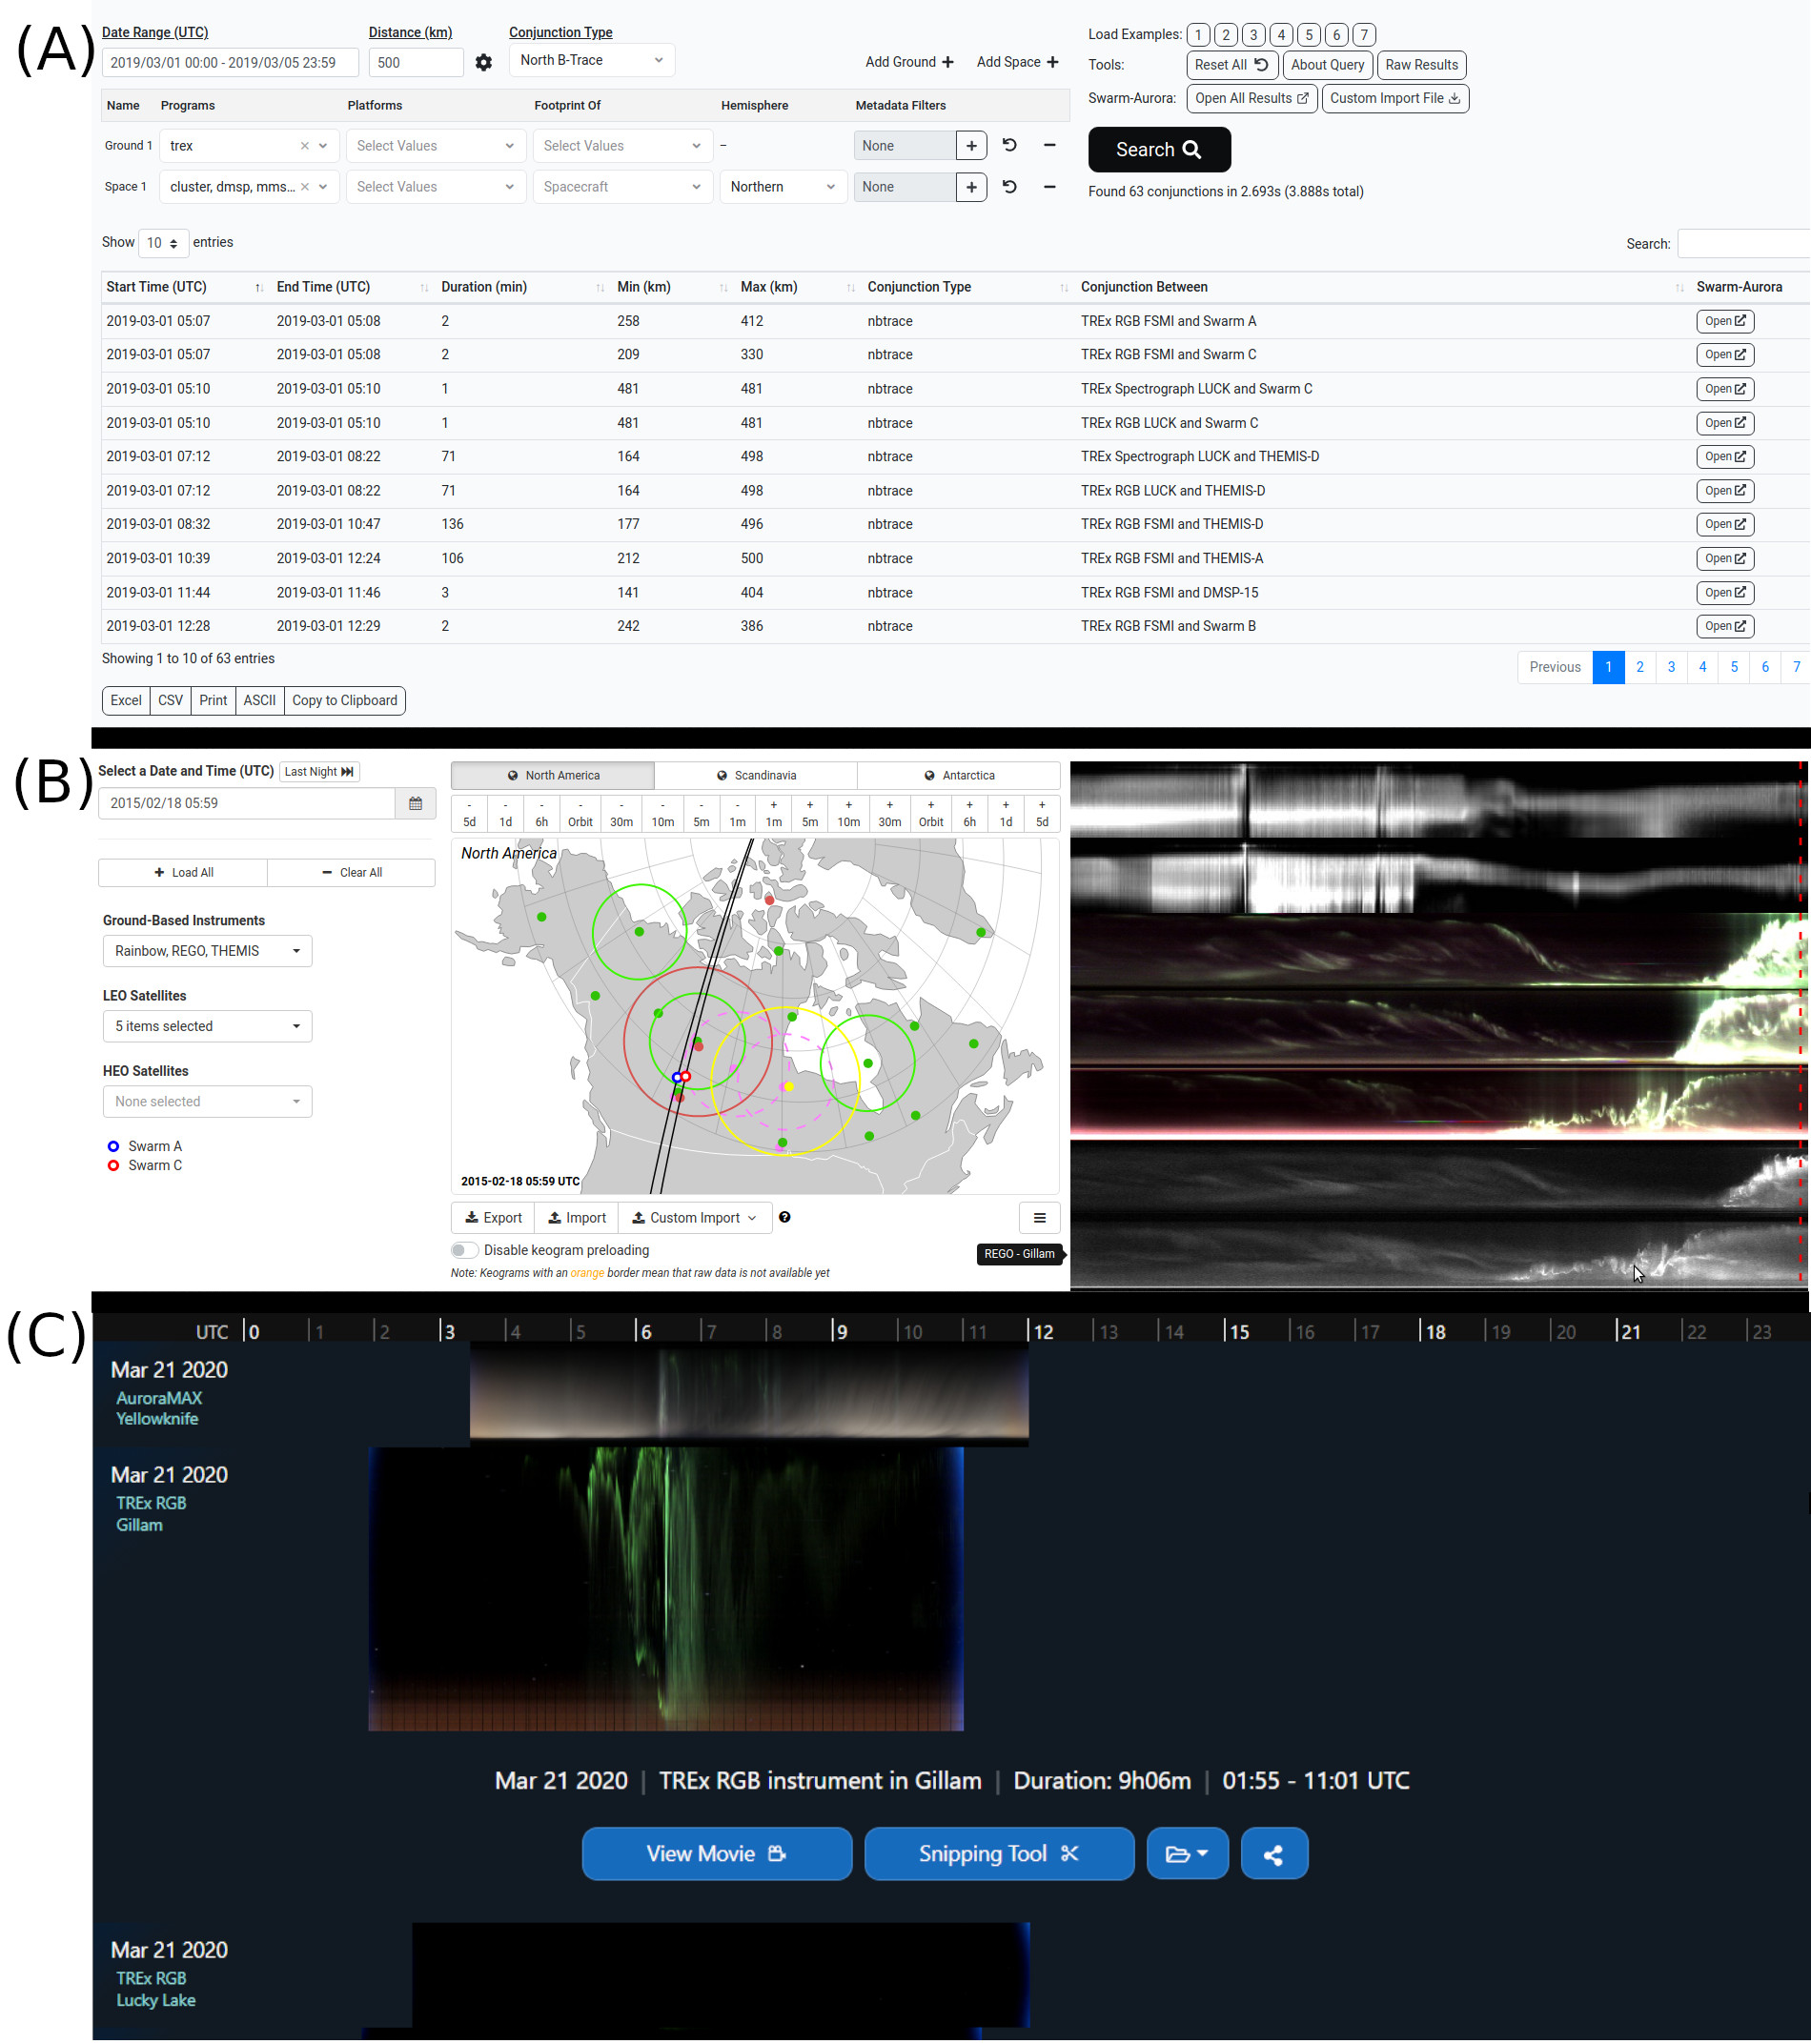
\includegraphics[width=0.9\textwidth]{figures/fig1.jpg}
    \caption{The \url{https://aurorax.space/} website. Panel (A) shows the conjunction finder with the customizable elements highlighted with the red rectangle. Panel (B) shows a detailed view of one of the conjunctions. Lastly, Panel (C) shows the Keogramist for three TREx ASIs on 21 March 2020. The Gillam keogram is expanded to show further options. }
    \label{fig1}
\end{figure}

\subsection{Virtual Observatory}

Besides the conjunction search, AuroraX allows users to easily browse through the summary data. The AuroraX Virtual Observatory provides interactive visualizations and data browsing interfaces to quickly navigate the vast amount of auroral data available in the platform. These interfaces are designed for browsing through the \textit{data repository} in a simple and efficient manner. AuroraX currently has two components to the Virtual Observatory: the Keogramist, and the Event Explorer.

As the name implies, the Keogramist (\url{https://aurorax.space/keogramist}) visualizes keograms---a highly compressed summary product for quickly analyzing ASI data. For the unfamiliar reader, a keogram corresponds to a time series representation of the luminosity along a single meridian. Typically, they are assembled by looping over every image and taking a vertical slice through the center of the image (or through a custom path such a path of a satellite). Objects in the sky such as auroral arcs, pulsating aurora, substorms, clouds, the moon, etc. have unique keogram signatures that allow for a quick interpretation. Keogramist presents keograms from any number of ASI instruments in the AuroraX data repository in a compact and visually-appealing interface. Figure \ref{fig1}(C) shows an example of the TREx keograms from 21 March 2020. Similarly, when a user identifies a day of interesting auroral activity, they can quickly view additional summary data such as timelapse movies. Keogramist also allows the user to filter the keograms displayed based on the \textit{data product} record metadata fields in the data repository. This could be as simple as the green-channel content in an RGB-based ASI, or more complex such as classifications derived from a machine learning model (e.g., pulsating aurora in the field-of-view).

Equally useful, the second component of the Virtual Observatory is the Event Explorer (\url{https://aurorax.space/eventExplorer}). Although this component  is still under development, it will allow users to see a 3D visualization of AuroraX ephemeris data with ground-based auroral images projected onto an interactive globe. This tool is designed to assist with visualizing auroral data and evaluating possible conjunctions using a more interactive and global interface. The auroral images are mapped to a 1024x512 grid covering $-180^\circ$ to $180^\circ$ longitude, and $-90^\circ$ to $90^\circ$ latitude (corresponding to $0.33^\circ$ longitude and $0.35^\circ$ latitude resolution), and visualized onto the globe. The grid format was first developed by NOAA and used as part of their 30-min auroral prediction OVATION model outputs \citep{Newell2010, Machol2012}. AuroraX has adopted this grid format to provide a global view of summary ASI data alongside representations of spacecraft geographic positions and magnetic footprints, provided by SSCWeb.

The Swarm-Aurora project was designed to facilitate and drive the use of Swarm \citep{Friis2006} in auroral science, and push Swarm beyond its primary mission objective to become a key instrument in auroral science research (\url{https://swarm-aurora.com}). In addition to AuroraX's Virtual Observatory components, the continued development of the Swarm-Aurora website has become a part of AuroraX’s priorities. One recent improvement has been the integration of AuroraX with Swarm-Aurora, allowing users to browse Swarm-Aurora using the AuroraX Conjunction Search results. In fact, the example conjunction search query shown in Fig. \ref{fig1}(A and B) was made by Swarm-Aurora. Lastly, architectural design changes were made to Swarm-Aurora to enhance the experience for users around the world, specifically optimizing loading times. Swarm-Aurora now operates on commercial cloud infrastructure in four regions; one in Calgary, two in the United States, and one in Europe. Adding more regions is trivial and can be done as the user base grows and are needed.

\subsection{PyAuroraX}
An important part of any platform like AuroraX is to allow users to leverage the data for use in their own scientific analyses and applications. To assist with these tasks, we developed software to interact with AuroraX using only a few lines of code. This is enabled by the AuroraX API and subsequent client libraries maintained by the project, one of which is PyAuroraX (\url{https://github.com/aurorax-space/pyaurorax}).

PyAuroraX allows users to interact with the AuroraX API and perform \textit{conjunction}, \textit{ephemeris}, and \textit{data product} searches using Python. For example, the \verb|pyaurorax.conjunctions.search()| function can be used to search AuroraX for conjunctions in the same way as the AuroraX Conjunction Search website. The below Python code shows how to perform a simple search, asking AuroraX to find all conjunctions between several instruments from the THEMIS ASI array and any Swarm spacecraft.

\begin{minted}{python}
import pyaurorax
import datetime

# define search parameters
start = datetime.datetime(2019, 1, 1, 0, 0, 0)
end = datetime.datetime(2019, 1, 3, 23, 59, 59)
ground_params = [
    {
        "programs": ["themis-asi"],
        "platforms": ["fort smith", "gillam"],
    }
]
space_params = [
    {
        "programs": ["swarm"],
        "hemisphere": ["northern"],
    }
]
distance = 500

# perform conjunction search
s = pyaurorax.conjunctions.search(start=start,
                                  end=end,
                                  distance=distance,
                                  ground=ground_params,
                                  space=space_params,
                                  verbose=True)
\end{minted}

Users can also retrieve other information from AuroraX such as data sources, \textit{ephemeris} records, \textit{data product} records, and data availability. All functions in PyAuroraX are also available for use with IDL programs by using the IDL-AuroraX library (\url{https://github.com/aurorax-space/idl-aurorax}). 

Documentation and examples are a key part of helping new users learn what is possible and provides a reference for more experienced users. To assist with this and ease the learning curve, AuroraX has developed a documentation website, available at \url{https://docs.aurorax.space}, with technical details about the platform, the metadata in it, and the various applications and tools available for use. Extensive examples and code snippets are available in the ``Developer Zone" to provide quick and simple uses of key programmatic tasks. The source code for this website is also available on Github alongside other open-source codebases within the AuroraX project (\url{https://github.com/aurorax-space/docs}). 

\section{Analyzing high-resolution ASI data using aurora-asi-lib}\label{aurora-asi-lib}
The final component of AuroraX is aurora-asi-lib, henceforth referred to, and imported as, asilib. It enables researchers to apply common data analysis tasks to the THEMIS and REGO ASI image data on a personal computer. Here we overview the main functions, while the online documentation at \url{https://aurora-asi-lib.readthedocs.io/} contains more examples, a tutorial, and a thorough API reference.

As we tour a few asilib functions, keep in mind that asilib is designed to manage the lower-level tasks. For example, if you want to load the image data via \verb|asilib.load_image()|, asilib will attempt to download the 1-hour Common Data Format (CDF) data if it is not already saved on your computer. Likewise, if you call \verb|asilib.plot_keogram()|, it will automatically load (and download if necessary) the ASI data before plotting it. For reference, Figs. \ref{fig2}-\ref{fig4} were made using the code in a Jupyter Notebook that is provided as supplemental material in both the ipynb and pdf formats.

\subsection{Plotting single images}
One common way to visualize all-sky images is with \verb|asilib.plot_fisheye()|. It plots the raw ASI images oriented with North at the top and East to the right of each image. The term fisheye comes from the fisheye lens that expands the imager's field of view to nearly $180^\circ$. Figure \ref{fig2}(A and C) show an example of an auroral arc observed concurrently by the THEMIS and REGO ASIs stationed at Rankin Inlet (RANK). By default the color map is automatically chosen: black-to-white for THEMIS and black-to-red for REGO. The default color scale is dynamically calculated using percentile logic described in the documentation.

The other common way to visualize images is by projecting the fisheye image onto a geographic map using \verb|asilib.plot_map()|. asilib uses the skymap files to map each pixel's vertices to a (latitude, longitude) point at an aurora emission altitude, typically assumed 110 km for THEMIS and 230 km for REGO \citep{Donovan2006b, Liang2016}. Figure \ref{fig2}(B and D) show the fisheye images mapped to 110 km altitude. By default, pixels that look at elevation $< 10^\circ$ are not mapped due to nearby obstructions and the stretching of pixels closest to the horizon. And lastly, \verb|asilib.make_map()| provides a default geographic map to project the images onto.

\begin{figure}
      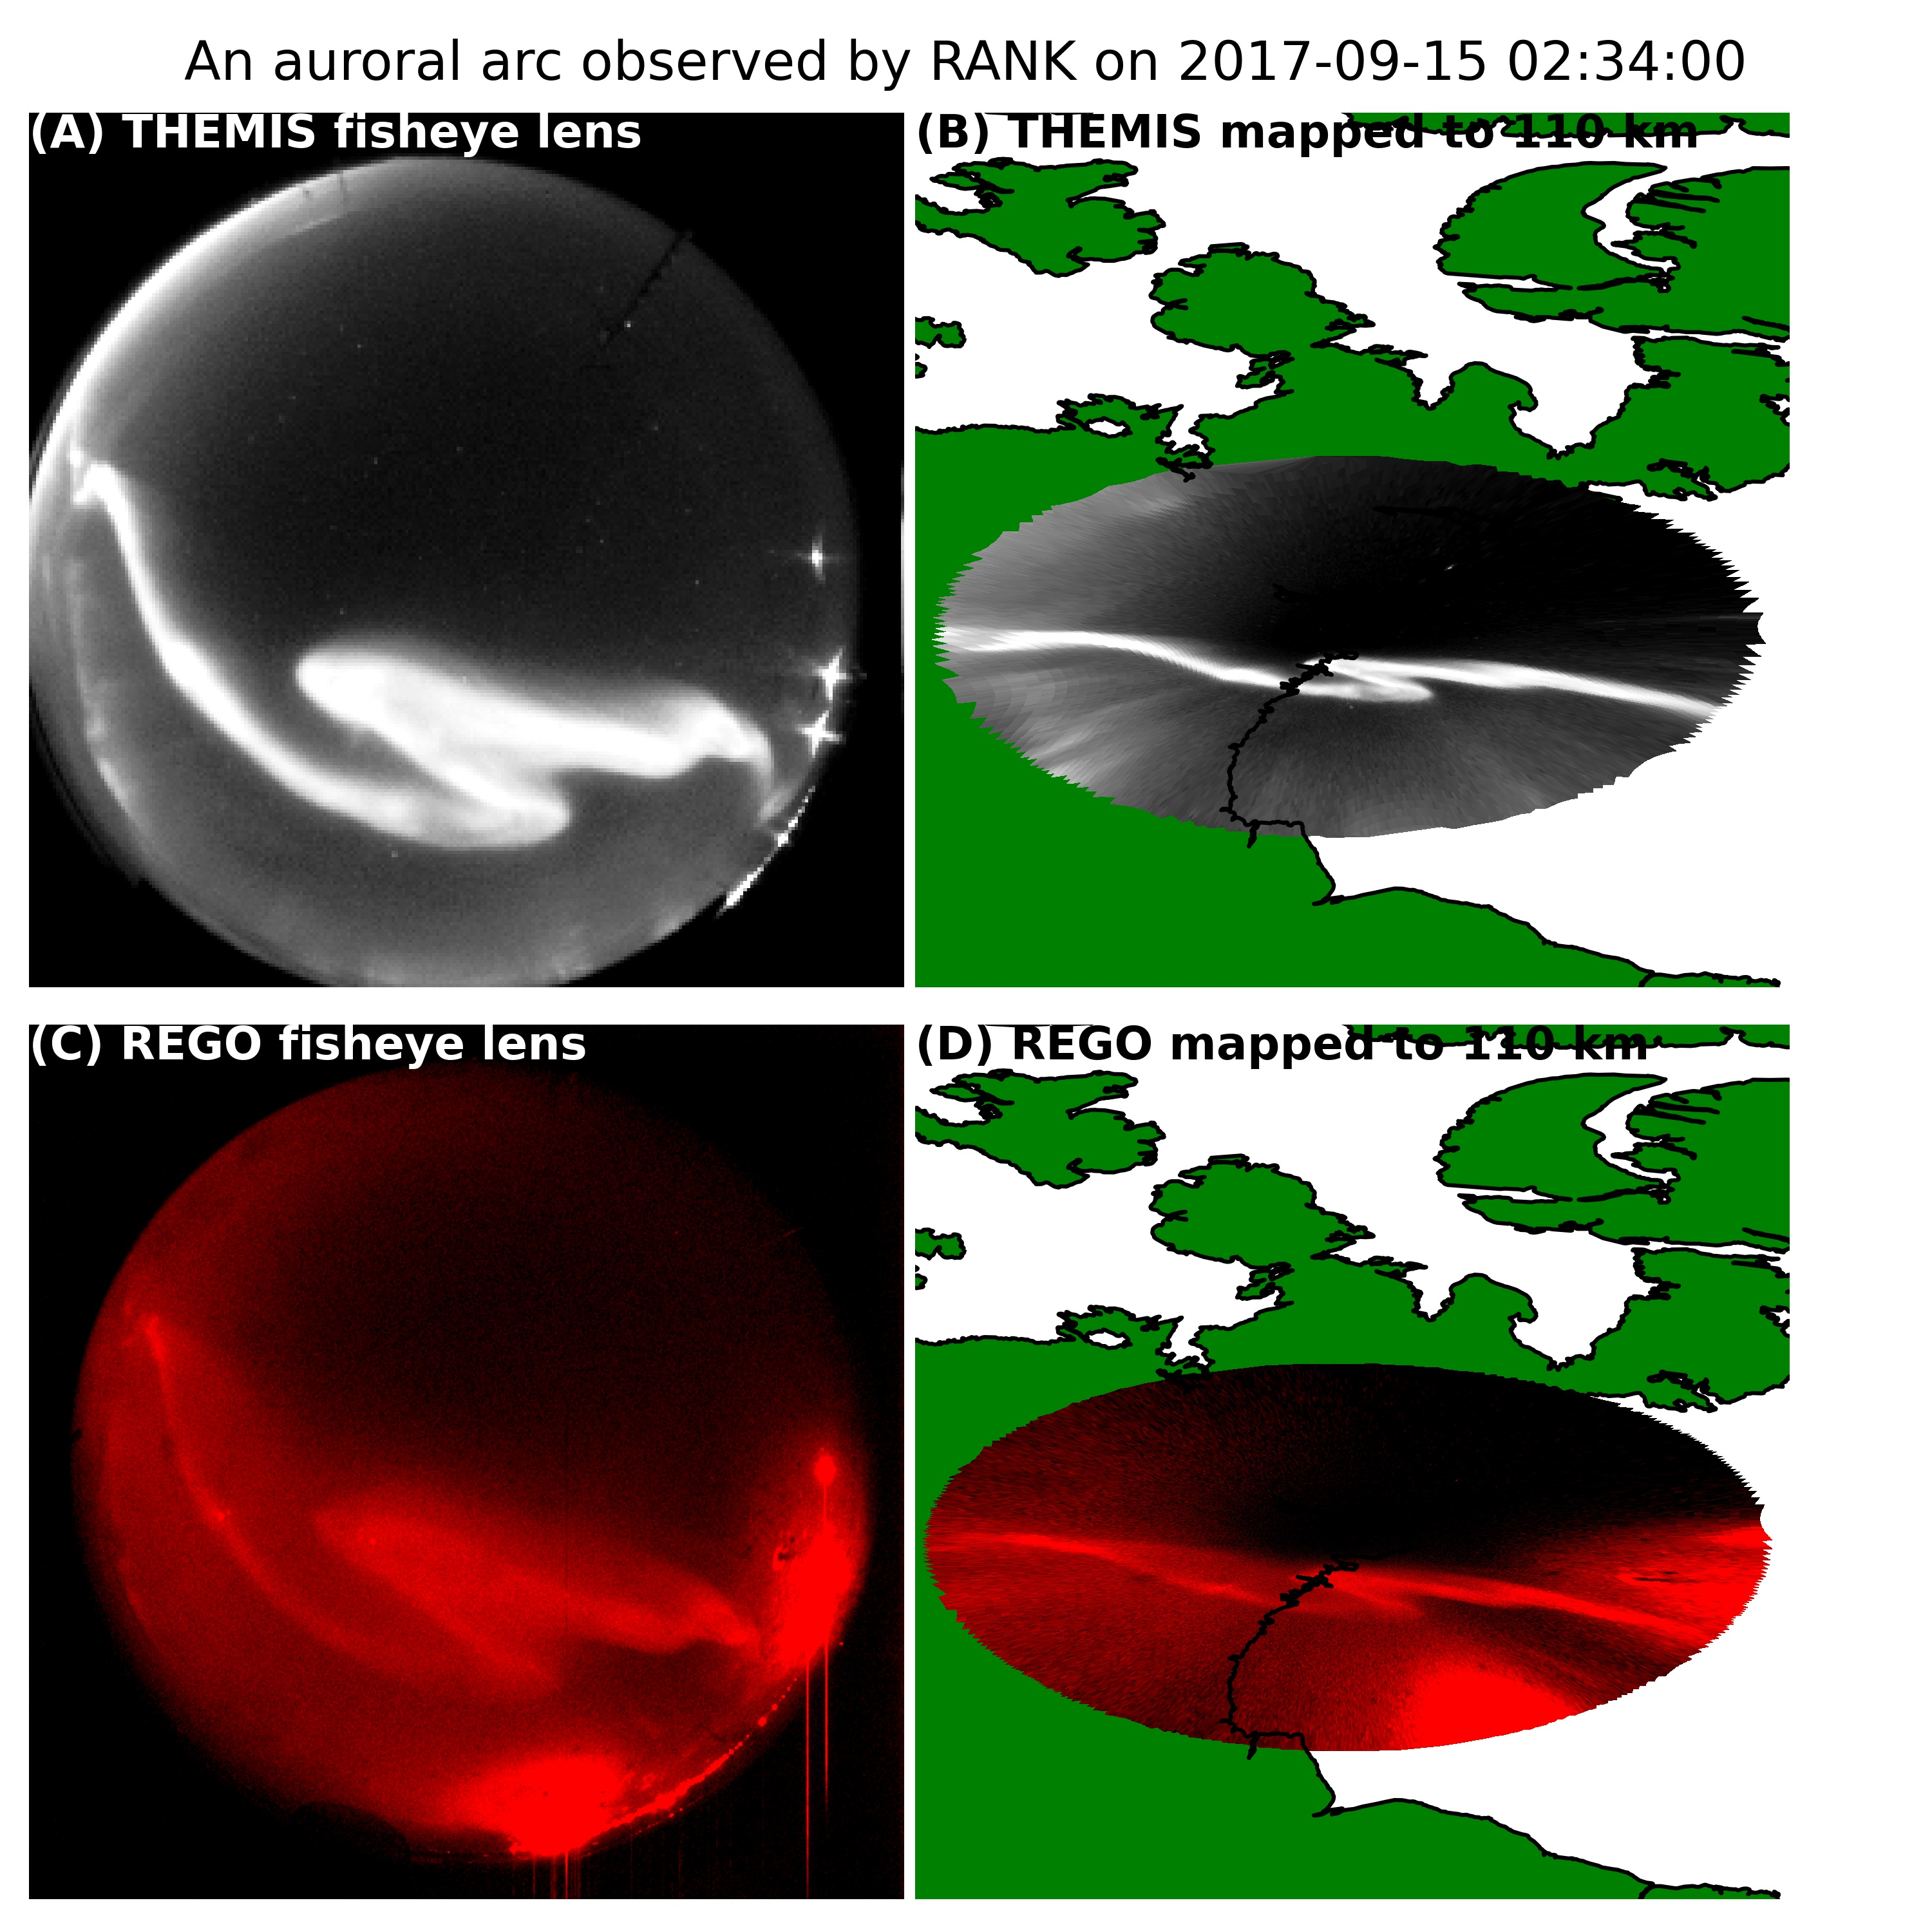
\includegraphics[width=\textwidth]{figures/fig2.jpg}
      \caption{An auroral arc observed simultaneously by the REGO and THEMIS imagers at Rankin Inlet, Canada. Panels (A) and (C) show the fisheye lens view, while panels (B) and (D) show the same images projected to the 110 km assumed aurora emission altitude. Only the pixels with elevation $>10^\circ$ are plotted.}
      \label{fig2}
\end{figure}

\subsection{Keograms}
You can make a keogram using the \verb|asilib.plot_keogram()| function that takes an optional \verb|map_alt| keyword argument. If \verb|map_alt| is not provided, the keogram's vertical axis is pixel index, as we show in Fig. \ref{fig3}(A). If a valid map altitude is provided, the vertical axis is geographic latitude as we show in Fig. \ref{fig3}(B). Lastly, by providing \verb|map_alt| and setting \verb|aacgm=True|, the vertical axis becomes magnetic latitude in the Altitude-adjusted corrected geomagnetic coordinate system (AACGM) \citep{Shepherd2014}. The latitude transformation between Fig. \ref{fig3}(A) and Fig. \ref{fig3}(B) is substantial---the low elevation pixels observe much wider regions of latitude, compared to the pixels at higher elevations.

\begin{figure}
      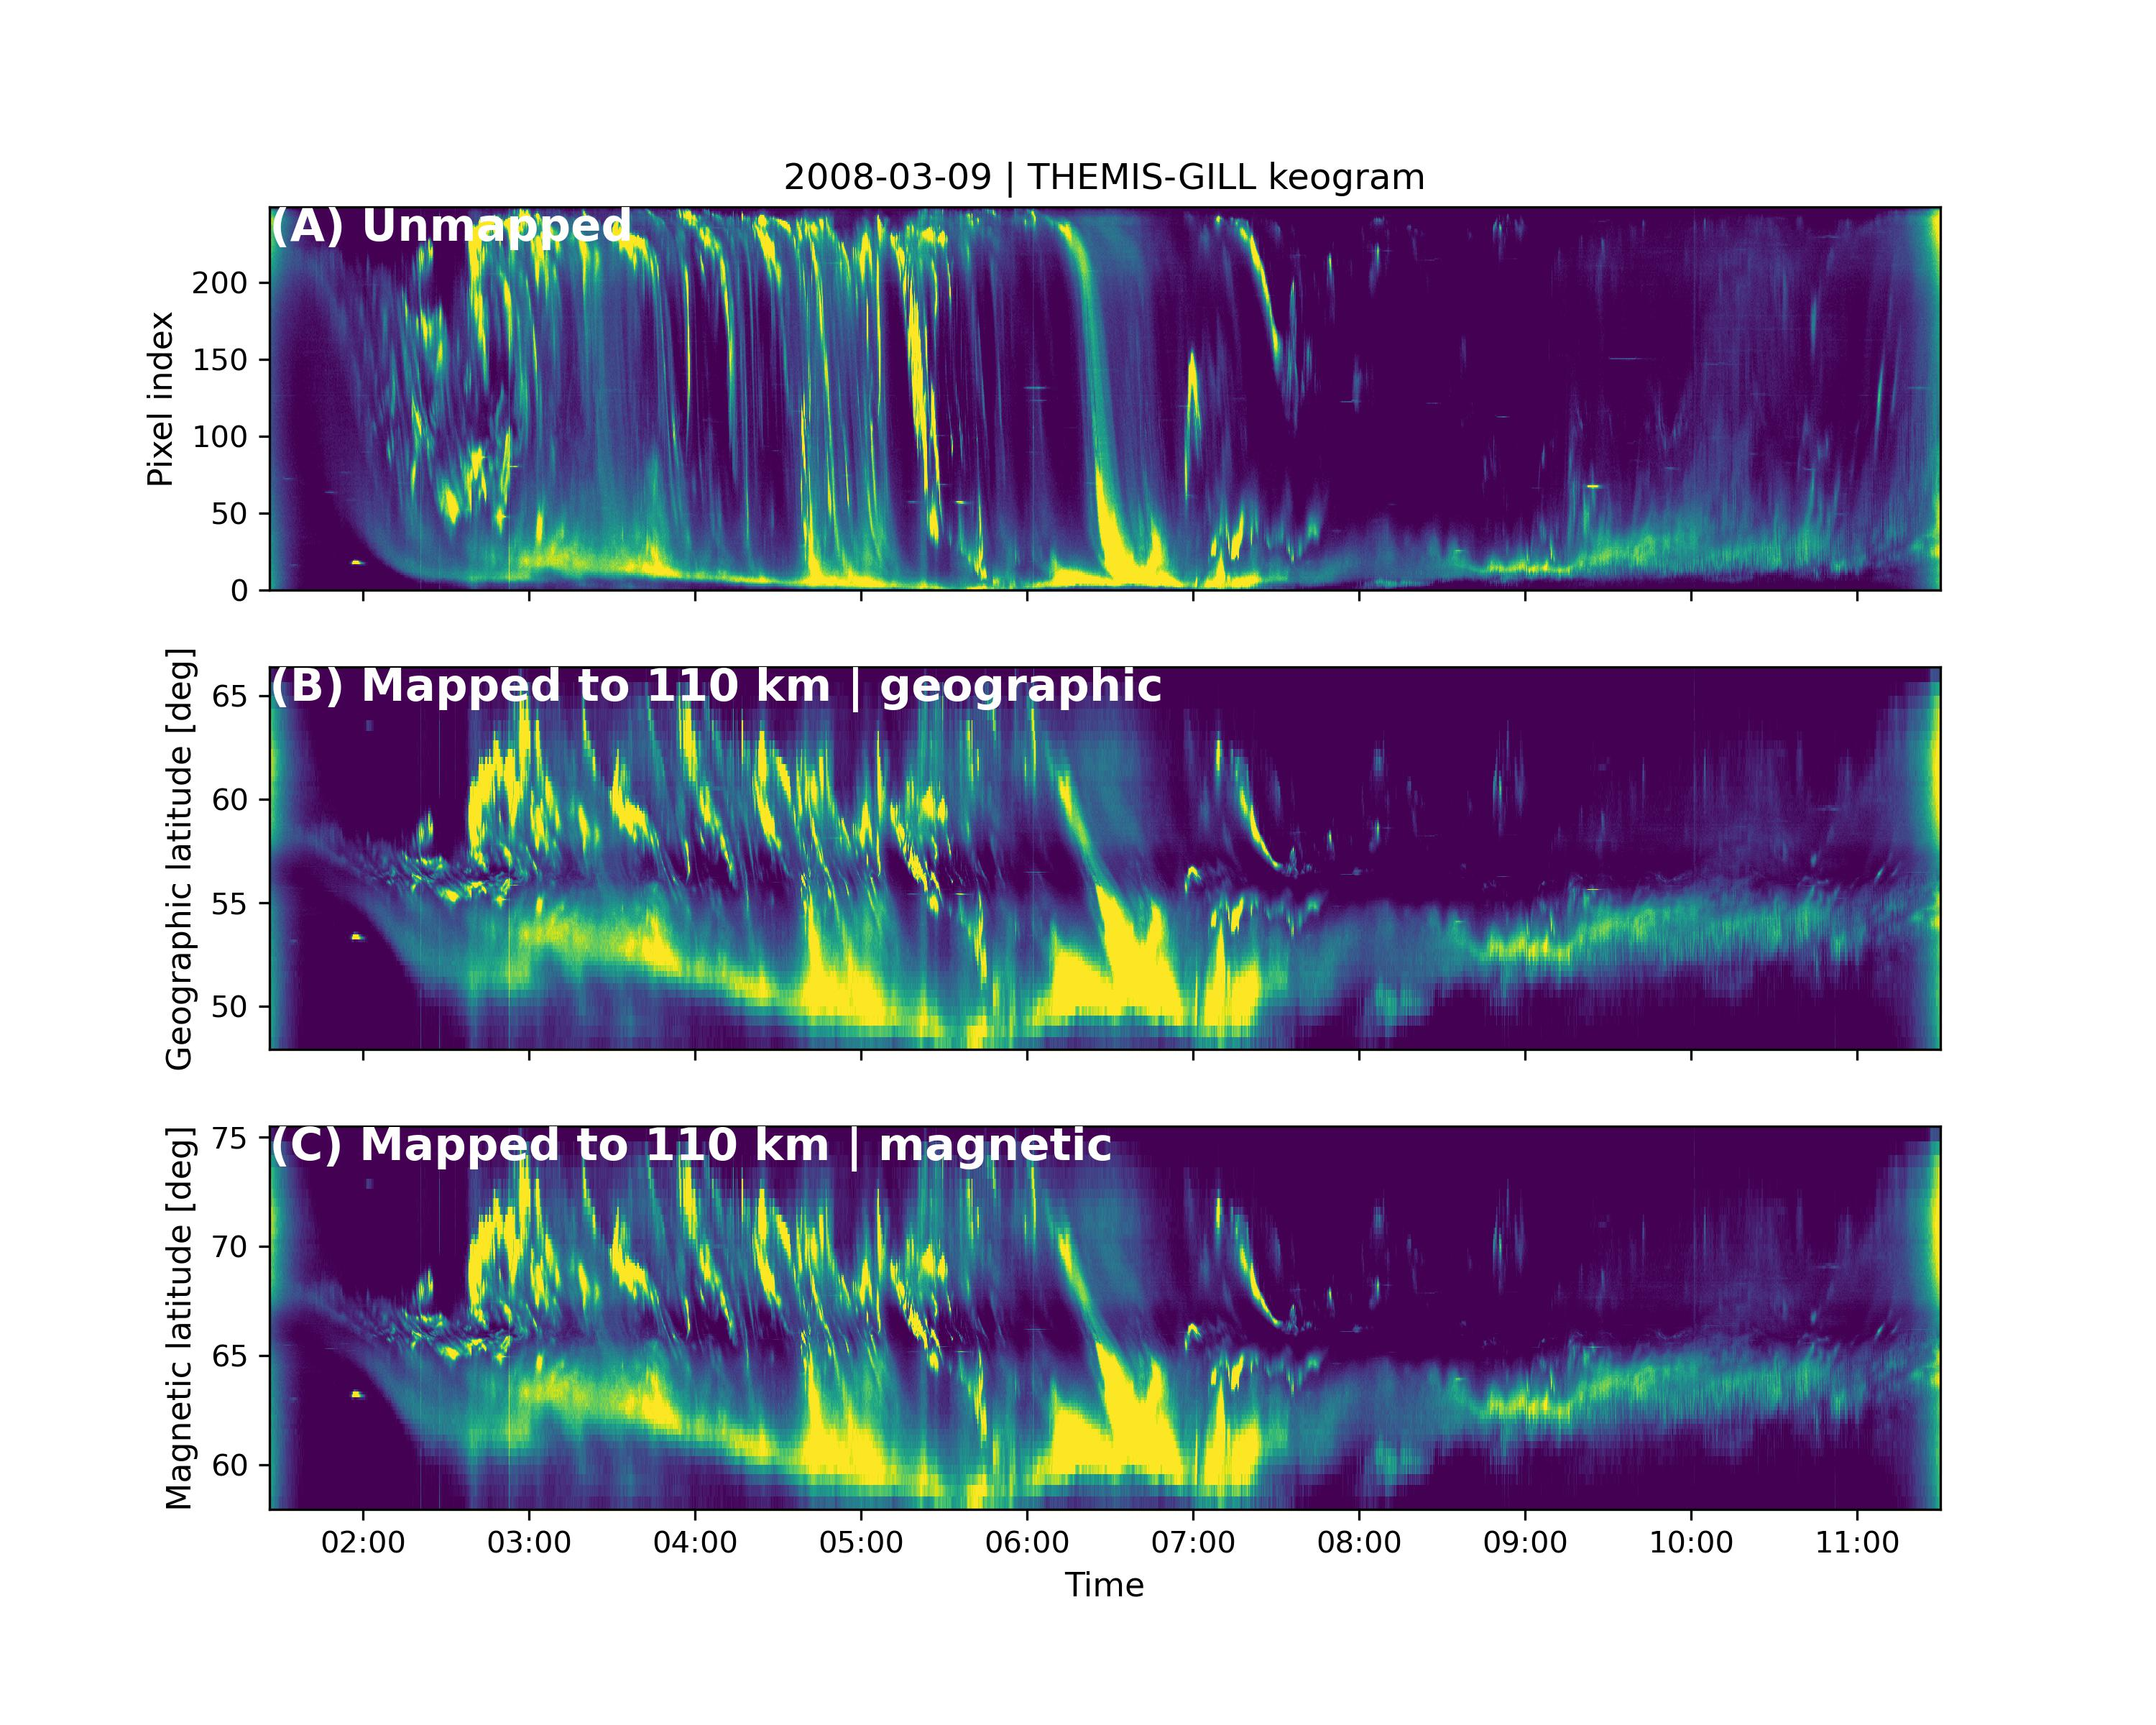
\includegraphics[width=\textwidth]{figures/fig3.jpg}
      \caption{A full-night keogram showing the dynamic aurora observed at Gillam, Canada on 9 March 2008. Panel (A) shows the unmapped keogram with the pixel index vertical axis, panel (B) shows the geographic latitude of the pixels mapped to 110 km altitude. Lastly, panel (C) shows the corresponding magnetic latitudes.}
      \label{fig3}
\end{figure}


\subsection{Animating Images}
asilib allows you to easily animate the fisheye and mapped images using \verb|asilib.animate_fisheye()| and \verb|asilib.animate_map()|. It first saves png images in a \\ \verb|asilib.config['ASI_DATA_DIR']/animations/images/| folder, and then animates them using the \verb|ffmpeg| library \citep{ffmpeg} . Animation S1 in the supporting document shows an example animation of auroral streamers.

Animating just the images is somewhat limiting. Thus, \verb|asilib| also includes \\ \verb|asilib.animate_fisheye_generator()| and \verb|asilib.animate_map_generator()| (which are technically coroutines) to allow the user to modify the animations as they are made. This is useful, for example, if you need to draw the satellite's location in each image.

\subsection{Conjunction analysis tools}
Currently, \verb|asilib| provides three functions that are useful for analyzing conjunctions: \verb|asilib.lla2footprint()|, \verb|asilib.lla2azel()|, and \verb|asilib.equal_area()|.

\verb|asilib.lla2footprint()| uses IRBEM-Lib (\citet{irbem}; requires a separate installation and compilation of the Fortran source code) to trace a satellite's position, in geographic (latitude, longitude, altitude) (LLA) coordinates, along a magnetic field line. This field line is defined using one of the magnetic field models that are supported by IRBEM. The primary use of this function is to map a satellite's location from, for example, 500 km altitude, to its magnetic footprint at the assumed auroral emission altitude (e.g. 110 km for THEMIS or 230 km for REGO as previously mentioned).

The next function is \verb|asilib.lla2azel()|. This function maps the satellite's footprint location, in LLA coordinates, to the ASI's (azimuth, elevation) coordinates (AzEl) using the skymap files. This function returns both the AzEl coordinates as well as the corresponding pixel indices.

Lastly, \verb|asilib.equal_area()| calculates a mask of pixels inside an auroral emission area---useful to calculate the mean auroral intensity (or another statistical quantity) in a physical area in the sky. The mask contains 1s inside of the area and \verb|numpy.nan| outside of it. You then multiply the image with the mask: the pixel intensities outside of the area are then \verb|numpy.nan| and unchanged inside the area. We chose to use \verb|numpy.nan| to ensure that the mean of the intensity is correctly applied---it will fail if you call \verb|numpy.mean(image*mask)|, but \verb|numpy.nanmean(image*mask)| will ignore NaNs and correctly calculate the mean intensity inside the area.

\subsection{Analyzing a conjunction}\label{satellite_conjunction}
In this example we combine the aforementioned analysis functions to calculate the mean auroral intensity surrounding the footprint of an artificial satellite during a conjunction with a THEMIS ASI. This satellite orbits at a 500-km altitude low Earth orbit. We will ultimately calculate the mean ASI intensity in a 20x20 km area at a 110 km altitude and animate the conjunction. Using an artificial satellite allows us to clearly exemplify how any satellite's footprint could be easily analyzed by asilib. 

For this example we use the satellite's location in LLA coordinates with time stamps that line up with the ASI times. In reality, the satellite and ASI time stamps are unlikely to line up, so you'll need to align the satellite's and ASI's time stamps.

Our analysis consists of three main steps:
\begin{enumerate}
    \item Trace the satellite's position along the magnetic field line to 110 km using  \verb|asilib.lla2footprint()|.
    \item Locate the satellite's footprint in the imager's field of view (azimuth and elevation coordinates) using \verb|asilib.lla2azel()|.
    \item Calculate the auroral intensity surrounding the satellite's footprint. We create a 20x20 km area mask using \verb|asilib.equal_area()| and use it to calculate the mean ASI intensity as a function of time (and satellite position).
\end{enumerate} These steps are implemented in the ``Figure 4" section of the \verb|asilib_figures| notebook.

Animation S2 shows the result of this conjunction analysis and Fig. \ref{fig4} shows a four-frame montage summarizing the animation. Fig. \ref{fig4}(A-D) show the fisheye lens images at the annotated time stamps. The satellite's footprint path is represented by the red line and the instantaneous footprint by the red dot. The yellow areas show the 20x20 km area around the footprint. And lastly, Fig. \ref{fig4}(E) shows the mean auroral intensity time series---clearly showing the auroral arc intensity between 2:33:30 and 2:34:15.

\begin{figure}
      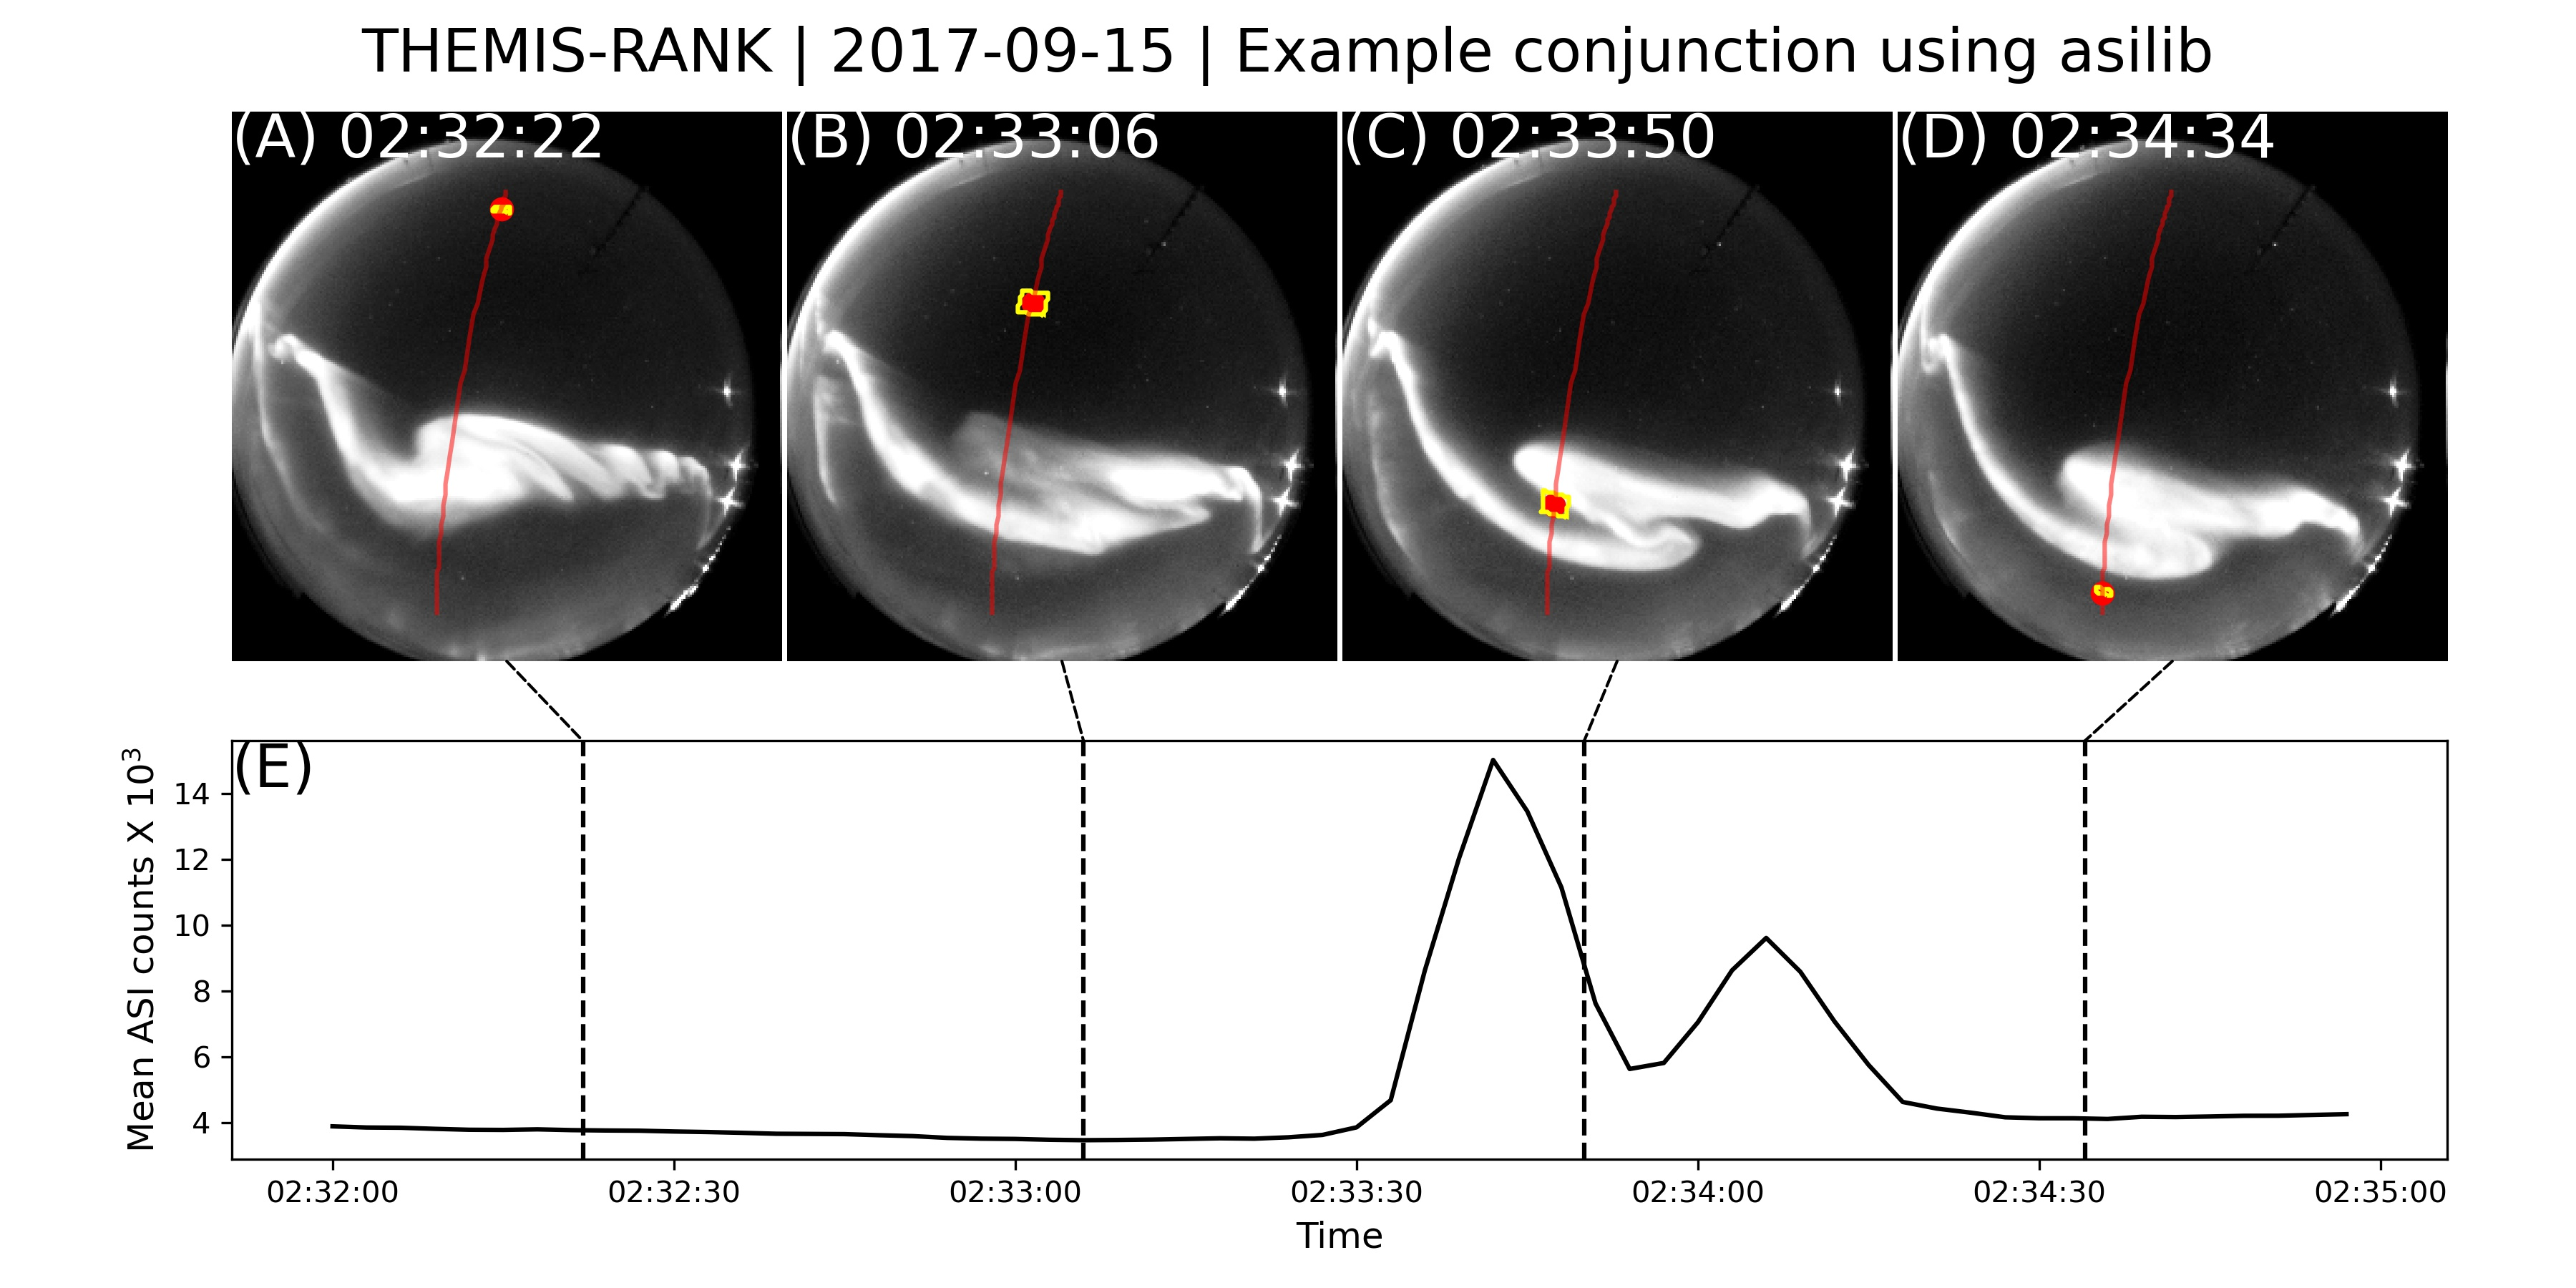
\includegraphics[width=\textwidth]{figures/fig4.jpg}
      \caption{A conjunction montage of Animation S2. Panels (A)-(D) shows the auroral arc evolution and the satellite's location. The red line is the satellite track and the red dot is its instantaneous position. The yellow quadrilateral bounds the pixels inside the a 20x20 km area surrounding the satellite's 110 km altitude footprint. Lastly, panel (E) shows the mean auroral intensity, as a function of time, and inside the yellow quadrilaterals. When the satellite passed through the arc between 2:33:30 and 2:34:15, the mean auroral intensity correspondingly intensified.}
      \label{fig4}
\end{figure}

\section{Quality Assurance}
We developed AuroraX, PyAuoraX, and aurora-asi-lib with usability, reliability, and maintainability at the forefront. Documentation is critically important to the survival and usability of software. The AuroraX documentation is hosted at \url{https://docs.aurorax.space/} and the asilib documentation at \url{https://aurora-asi-lib.readthedocs.io/}. There you will find installation instructions, examples, comprehensive tutorials, and API references.

The source code for AuroraX, PyAuroraX, and asilib  is open source and hosted on GitHub. The two Python libraries are also cataloged on Zenodo and can be installed from the Python Packaging Index (PyPI; install using the \textit{pip} command). On GitHub you can submit an Issue for bugs or feature requests, and contribute with a Pull Request.  

To ensure code stability, the codebases for both Python libraries include tests suites that you can run locally and are automatically executed using GitHub Actions every time a change is pushed to the repository. These comprehensive tests check and warn of any software bugs or changes in function behaviour over the course of further development and maintenance.


\section{Conclusion}
The AuroraX website, PyAuroraX, and aurora-asi-lib tools provide the auroral science community with a simple and robust set of analysis tools to enable system-level auroral science. As we demonstrated, these tools provide an end-to-end analysis solution for using auroral data. We described one such solution: to identify and analyze conjunctions. We showed how you can use the AuroraX Conjunction Search website or PyAuroraX to identify and filter conjunctions between a number of ASIs and spacecraft. We then use aurora-asi-lib to quantify the auroral intensity at the satellite's footprint during a conjunction. This example is just one way that AuroraX can help you quickly sift through an immense volume of ASI data to uncover new physics in a significantly less amount of time than was previously possible.

In the near future we will expand AuroraX’s data repository by including more ASI arrays, satellites, and informative metadata filters. Furthermore, TREx and other ASIs will be added to aurora-asi-lib by the current development team and the community. The continued success and usability of AuroraX depends on community contributions. We encourage an open science approach, and look forward to working more broadly within the auroral research community.


\section*{Conflict of Interest Statement}
The authors declare that the research was conducted in the absence of any commercial or financial relationships that could be construed as a potential conflict of interest.

\section*{Author Contributions}
ED, ELS, and DC designed and developed the AuroraX platform and PyAuroraX. AJH, KRM, and IT assisted MS with developing aurora-asi-lib. MS, BGL, DC, and ED wrote the manuscript. ED, ELS, and DC provided the THEMIS and REGO ASI data and expertise.  All authors contributed to manuscript revision, read, and approved the submitted version

\section*{Funding}
MS and BGL acknowledge the support provided by the NASA Postdoctoral Program at the NASA's Goddard Space Flight Center, administered by Oak Ridge Associated Universities under contract with NASA. BGL was also supported by the NASA competed Internal Scientist Funding Model (ISFM) on Mesoscale Magnetospheric Dynamic. AJH was supported in part by the Goddard ISFM which funds the Space Precipitation Impacts team with grant HISFM21. ED, ELS, and DC acknowledge the AuroraX funding sources: the Canadian Foundation for Innovation (CFI), the Province of Alberta, the Technical University of Denmark (DTU, Swarm DISC Program), and the Canadian Space Agency.

\section*{Acknowledgments}
The authors acknowledge all of the scientists, technicians, and engineers who designed, built, and maintain these ASI arrays. The UCalgary team acknowledges the AuroraX, REGO ASI and THEMIS ASI funding agencies and thanks them for their continued support. The UCalgary team also acknowledges the University of Alberta and RGP Consulting for their work on AuroraX. 

\section*{Data Availability Statement}
The datasets and code presented here can be found in the following links.
\begin{itemize}
    \item AuroraX: \url{https://aurorax.space/} and \url{https://github.com/aurorax-space}
    \item AuroraX documentation: \url{https://docs.aurorax.space}
    \item aurora-asi-lib: \url{https://aurora-asi-lib.readthedocs.io/en/latest/}
    \item THEMIS: \url{https://data.phys.ucalgary.ca/sort_by_project/THEMIS/asi/}
    \item REGO: \url{https://data.phys.ucalgary.ca/sort_by_project/GO-Canada/REGO/}
\end{itemize}

\section*{Contribution to the Field Statement}
\noindent The aurora is a ubiquitous light spectacle that has been observed in the polar regions for millennia. The regional scale of the aurora has led to the recent development of numerous all-sky imagers (ASIs)---and arrays of imagers---that continuously take images every night. The large volume of images has quickly become unmanageable by any single group of scientists, leading to datasets that are at best fragmented on the internet, and at worst hidden from the public. The AuroraX project (\url{https://aurorax.space/}) aims to address this problem with a centralized metadata search platform that combines auroral imaging datasets into one easily used resource. This project consists of various tools including a data repository, a search engine, web-based search and analysis interfaces, and software-driven programmatic interfaces (ie. APIs, client libraries such as PyAuroraX). Additionally, the Python library aurora-asi-lib provides the ability to easily analyze high-resolution auroral data from two key ASI arrays – THEMIS and REGO. Together, these tools provide an important improvement to the accessibility and usability of all-sky imager data for auroral science.

\bibliographystyle{Frontiers-Harvard} 
\bibliography{refs}
\end{document}